\documentclass{beamer}
\usetheme{Frankfurt}
\usepackage{physics}
\usepackage[]{graphicx} 
\usepackage[]{amsmath} 

\title{Quantum Spin Hall Effect}
\author{Chia-Wei Wei}
\date{June 28 2021}
\institute[NTHU] % Your institution as it will appear on the bottom of every slide, may be shorthand to save space
{National Tsing Hua University\\} % Your institution for the title page}


\begin{document}
  
\begin{frame}
\maketitle
\end{frame}

\begin{frame}
\frametitle{Overview}
\tableofcontents
\end{frame}
%------------------------------------------------------------------------
\section{Haldane's graphene model}
\begin{frame}
\frametitle{Haldane's graphene model}
\begin{figure}[htpb]
  \centering
  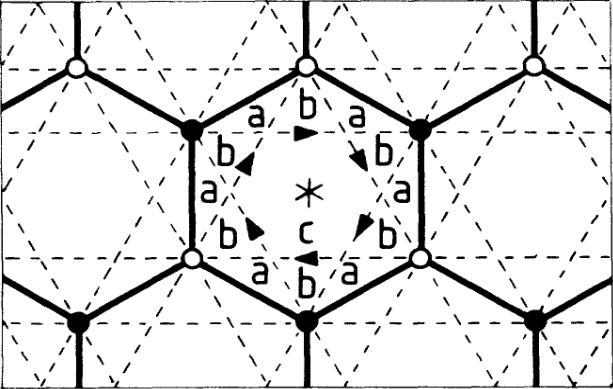
\includegraphics[width=0.7\linewidth]{graphene.png}
  \caption{The honeycomb model showing nearest neighbor hopping (solid lines)
  and second neighbor hopping (dash lines), two sublatices are charaterized
by open and soilid points.}%
  \label{fig:graphene}
\end{figure}
\end{frame}

\begin{frame}
  \frametitle{Hamiltonian}
In 1988, Duncan Haldane proposed the scenario for the quantum Hall state
which absence the magnetic field. In his paper, he add a periodic staggered 
local magnetic-flux density $\textbf{\emph{B}(r)}$ in the ${\bf \hat{z}}$
direction normal to the 2D plane, but with $\emph{zero total flux}$ through
the unit cell. 

\begin{equation*}
\begin{split}
  H = &[- t\sum_{\left<i,j\right>}a^{\dagger}_{i}b_{j} + \frac{M}{2}
  \sum_{i=1} (a^{\dagger}_{i}a_{i} - b^{\dagger}_{i}b_{i})] + h.c.\\ 
  & + t_{2}\sum_{\left<\left<i,j\right>\right>}[e^{i\varphi}a^{\dagger}_{i}a_{j} +
  e^{-i\varphi}b^{\dagger}_{i}b_{j}] 
\end{split}
\end{equation*}
where the $t$ and $t_{2}$ are hopping amplitude, the $\varphi$ is the phase
caused by the total fluxes threading through the second hopping.
The third term means that second neighbor hopping term, 

\end{frame}

\begin{frame}
  \frametitle{the conductance of this system}
The conclusion of this paper is, while the system is in presence of
magnetic flux, the Chern number is not zero which shows the topological
property which same as the quatun Hall effect system. Haldane calculate the
Hall conductane when system break the time reversal symmetry which is

\begin{equation*}
  \sigma_{H} = \frac{\partial \rho}{\partial B_{z}} \bigg\rvert_{\mu} =
  \frac{\nu e^{2}}{h} \bigg\rvert_{\nu = 1} 
\end{equation*}
\end{frame}

\begin{frame}
 \begin{figure}[htpb]
  \centering
  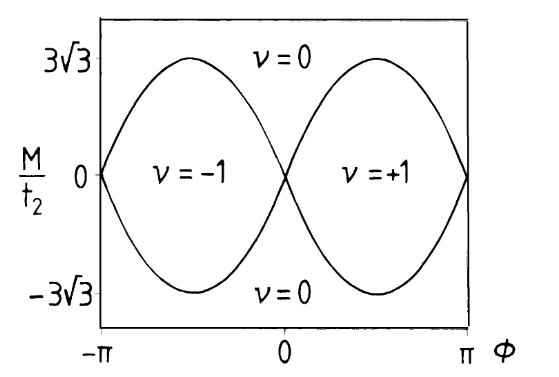
\includegraphics[width=0.8\linewidth]{cherm.png}
  \caption{By tuning the parameter in the Hamiltonian
  the system would show the zero-field quatum Hall effect phases ($\nu=\pm
1$, where $\sigma^{xy}=\nu \frac{e^2}{h}$)}%
  \label{fig:cherm}
\end{figure}
\end{frame}

%---------------------------------------------------------------------------
\section{The proposal of QSHE by Kane and Mele}
\begin{frame}
  \frametitle{The proposal of QSHE}
In 2005, Kane and Mele proposed the idea which considers the strong spin 
orbital interaction in the sigle layer graphene. They found that spin and
charge current can be transported in the gapless edge states. The
Hamiltonian in this model whcih can be written as
\begin{equation*}
{\cal H}_0 = -i\hbar v_F \psi^\dagger(\sigma_x\tau_z\partial_x +
\sigma_y\partial_y)\psi.
\end{equation*}

The SO interaction allows for a new terms which doesn't break the time
reversal symmetry.
\begin{equation*}
{\cal H}_{SO} = \Delta_{so} \psi^\dagger \sigma_z\tau_z s_z \psi.
\end{equation*}

Here $s_z$ is Pauli matrix representing the electron's spin,which respects
all of the symmetry of graphene

$\sigma_z = \pm 1$ describing states on the $A(B)$ sublattice and
$\tau_z = \pm 1$ describing states at the $K(K')$ points. 
\end{frame}

\begin{frame}
They consider the Rashba term which the mirror symmetry is broken. 

\begin{equation*}
{\cal H}_R = \lambda_R \psi^\dagger (\sigma_x\tau_z s_y - \sigma_y
s_x)\psi.
\end{equation*}

If Rashba term is zero, there leads to an energy gap with $E(\bf
q) = \pm\sqrt{(\hbar v_F q)^2 + \Delta_{so}^2}$. For $0<\lambda_R<\Delta_{so}$ the energy gap $2(\Delta_{so}-\lambda_R)$
remains finite.  For $\lambda_R>\Delta_{so}$ the gap closes, and the
electronic structure is that of a zero gap semiconductor with
quadradically dispersing bands.


\end{frame}

\begin{frame}
\begin{itemize}
  \item $\sigma_z\tau_z s_z$ is different from the gap that
would be generated by the staggered sublattice potentials,
$\sigma_z$ or $\sigma_z s_z$.

\item The spin dependent Hamiltonian which violet the time reversal symmetry are
equivalent the Haldane's model with spinless electrons which periodic
magectic field with no net flux.

\item Spin would gives rise a gap where has a opposite signs at $K$ and $K'$
points.
\end{itemize}
\end{frame}

\begin{frame}
 In this system we can computed the quantized Hall conductance which can be
 $\sigma_{xy}=\pm e^2/h$. Since the SO interaction would cause the opposite
 sign of gaps for opposite spins which induce the opposite current for the
 opposite spins. Spin current is ${\bf J}_s = (\hbar/2e)({\bf J}_\uparrow-
 {\bf J}_\downarrow)$ characterized by a quantized spin Hall conductivity

\begin{equation*}
\sigma^s_{xy}={e\over{2\pi}}.
\end{equation*}

\end{frame}

\begin{frame}
\frametitle{Band structure after adding Rashba term}
   \begin{figure}[htpb]
  \centering
  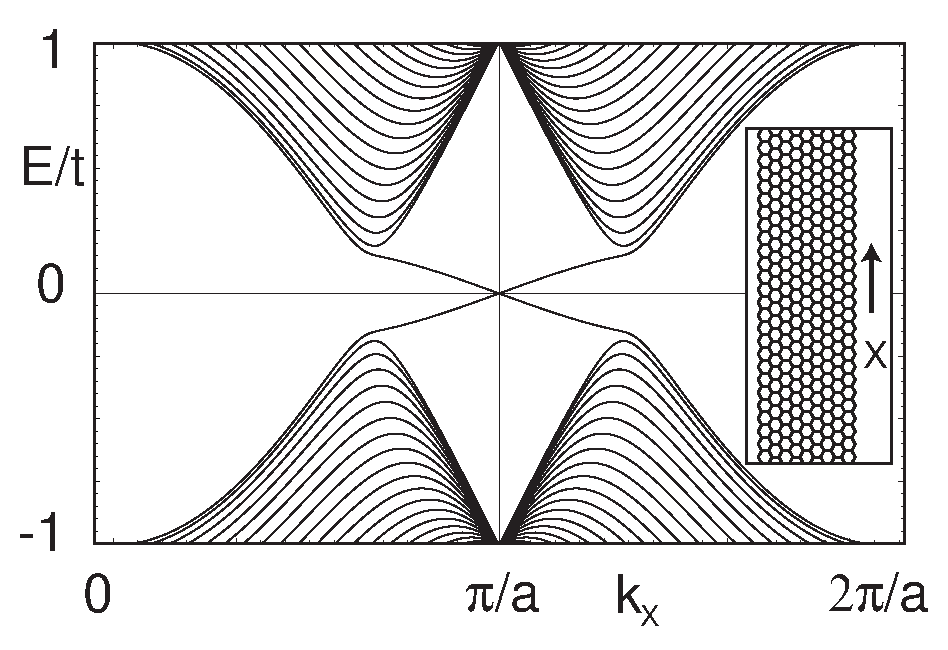
\includegraphics[width=0.7\linewidth]{fig1.eps}
  \caption{In this figure we would see that there is crossing at
  $\pi/a$ which is robust protected by the time revesal symmetry
follows the Kramer theorem. We can image that the QSHE can be caused by two
copies of Haldane's model which preserves the time reveseral symmetry which
is broken in Haldane's.}%
  \label{fig:fig1}
\end{figure}

\end{frame}

%---------------------------------------------------------------------------
\section{The QSHE of Bernevig and Zhang}
\begin{frame}
\frametitle{The QSHE of Bernevig and Zhang}
Bernevig and Zhang proposed that the SO is not easy to realized in term of
electric field, but there is another way which the shear strain gradients
can play a similar role.

For the purpose, we use replace the electric field by using the shear
strain which is,
\begin{equation*} \label{strainelectricfieldanalogy}
\epsilon_{xy} \leftrightarrow E_z;\;\;\; \epsilon_{xz} \leftrightarrow
E_y;\;\;\;\epsilon_{yz} \leftrightarrow E_x
\end{equation*}
After this replacement our Hamiltonian can be written as,
\begin{eqnarray*}
& H = \frac{p^2}{2m} + B tr{\epsilon} +\frac{1}{2}
\frac{C_3}{\hbar}
[ (\epsilon_{xy} p_y - \epsilon_{xz} p_z) \sigma_x  \nonumber \\
& +(\epsilon_{zy} p_z - \epsilon_{xy} p_x) \sigma_y + (\epsilon_{zx}
p_x - \epsilon_{yz} p_y) \sigma_z ]
\end{eqnarray*}
For GaAs, the constant $\frac{C_3}{\hbar} = 8 \times
10^5 m/s$.
\end{frame}

\begin{frame}
Bervenig and Zhang consider that system in quantum well in $xy$ plane which
is parabolic and Hamiltonian with the strain fonfiguration can becomes:

\begin{equation*}
H= \frac{p_x^2 + p_y^2}{2m} + \frac{1}{2} \frac{C_3}{\hbar}g (y p_x
- x  p_y)\sigma_z + D(x^2 + y^2)
\end{equation*}

Then make the change of variable, our Hamiltonian can be $H =
(1/2m) (\vec{p} - e \vec{A} \sigma_{z})^2$ with ${\vec{A} =
(m C_3 g/2 \hbar e) (y, -x, 0)}$. This Hamiltonian is equivalent the
charge in the uniform magnetic field which two different spin experience
the opposite directions of magnetic field.

\end{frame}

\begin{frame}
\frametitle{Hamiltonian}
 In this Hamiltonian the $s_z$ is a good quantum number, therefore our
 Hamiltonian can be written as:
\begin{eqnarray*}
& H = \left(%
\begin{array}{cc}
  H_{\uparrow} & 0 \\
  0 & H_{\downarrow} \\
\end{array}%
\right) \nonumber\\ & H_{ \downarrow , \uparrow} =
\sqrt{\frac{D}{2m}} [p_x^2 + p_y^2 + x^2+ y^2 \pm R(x p_y - y p_x)]
\end{eqnarray*}

Then choosing the $z = x+ i y$, we obtain two
sets of raising and lowering operators:
\begin{eqnarray*}
& a = \partial_{z^\star} + \frac{z}{2}, \;\;\; a^\dagger = - \partial_z + \frac{z^\star}{2} \nonumber \\
& b = \partial_{z} + \frac{z^\star}{2}, \;\;\; b^\dagger = -
\partial_{z^\star} + \frac{z}{2}
\end{eqnarray*}
\end{frame}

\begin{frame}
After introducing the raising and lowering operators, our Hamiltonain can
be:
\begin{equation*}
H_{\downarrow, \uparrow} =2 \sqrt{\frac{D}{2m}} \left[(1 \mp
\frac{R}{2} ) a a^\dagger + (1 \pm \frac{R}{2}) b b^\dagger  + 1
\right]
\end{equation*}

The eigenstates of this system are harmonic oscillators
$|m,n\rangle = (a^\dagger)^m (b^\dagger)^n |0,0\rangle$ of energy is
\begin{equation*}
  E^{\downarrow, \uparrow}_{m,n} = \frac{1}{2} \sqrt{\frac{D}{2m}}
\left[(1 \mp \frac{R}{2} ) m + (1 \pm \frac{R}{2}) n + 1 \right]
\end{equation*}

Following discussion we focus on $R = 2$ ($R =
\frac{1}{2} \frac{C_3}{\hbar} \sqrt{\frac{2m}{D}} g$) where there is no 
addtional static potential within Landau level
\end{frame}

\begin{frame}
\begin{itemize} 
  \item For the spin up electron, the vicinity of $R \approx 2$ is 
characterized by the Hamiltonian $H_{\uparrow} = (1/2)(C_3/\hbar) g (2 a a^\dagger + 1) $ 
with the LLL wave function
$\phi^\uparrow_n(z) =\frac{z^n}{\sqrt{\pi n! } }\exp(\frac{-z
z^\star}{2})$. These up spin electrons
are the chiral, and their charge conductance is quantized in units
of $e^2/h$.
\item The spin down is same as spin up just replce $a a^\dagger$ by
  $bb^\dagger$. These electrons are also chiral, but conductance is opposite
  of sign of spin up one.
\end{itemize}
\end{frame}

\begin{frame}
  \frametitle{Figure describes by Hamiltonian}
  \begin{figure}[htpb]
  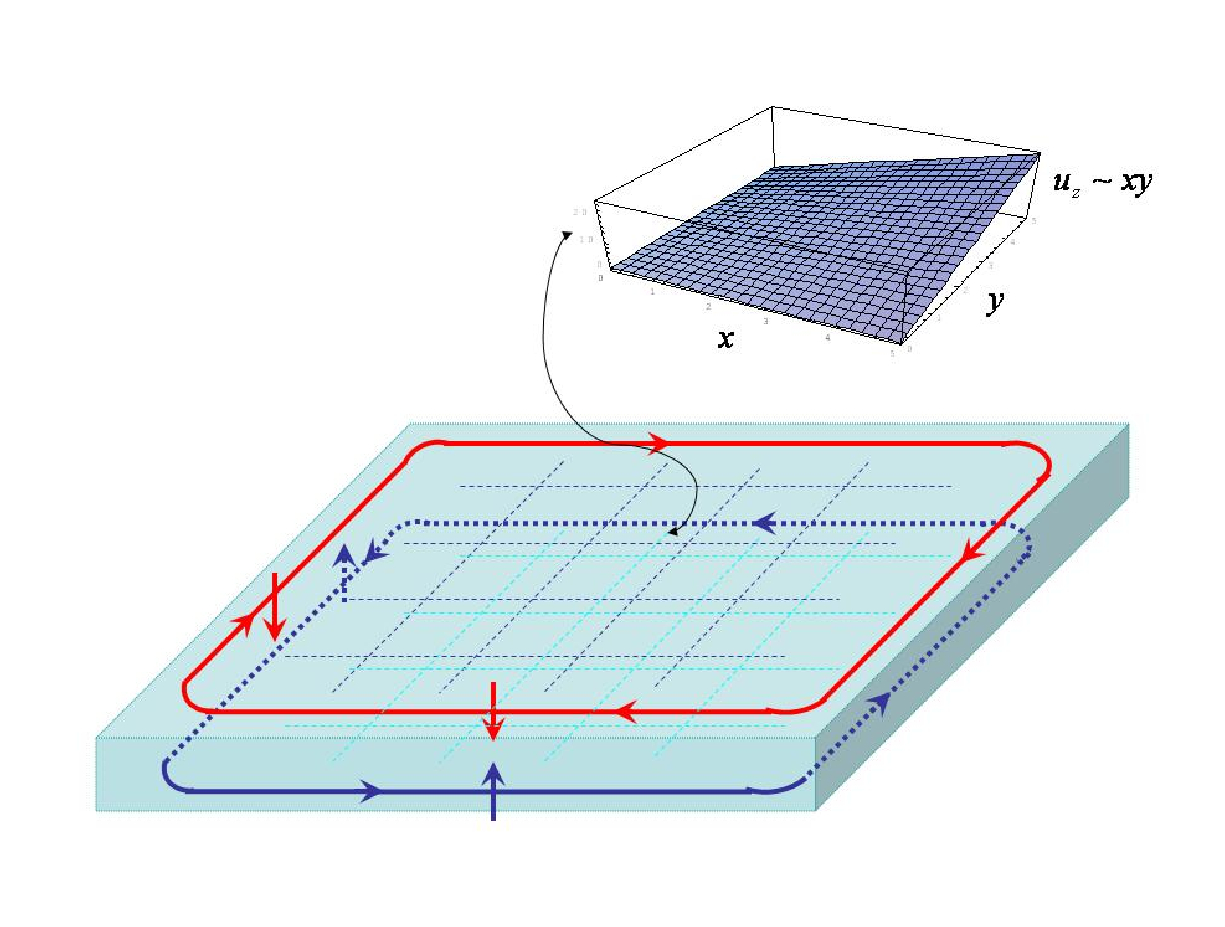
\includegraphics[scale=0.35]{edgecurrent.eps}
  \caption{Spin up and down electrons have opposite chirality as
they feel the opposite spin-orbit coupling force. Total charge
conductance vanishes but spin conductance is quantized. The inset
shows the lattice displacement leading to the strain
configuration.}
 \label{fig:edgecurrent}
  \end{figure} 
\end{frame}

\begin{frame}
In the previous slide's figure the totoal charge conductance is zero for 
the whole system. But, the time reversal smmetry reserves the direction of 
the "effective" magnetic, and interchanges the laers at the same time. 
This means that the spin Hall conductance is remain finite which is 
quantized in units of $2 \frac{e^2}{h} \frac{\hbar}{2e}=2\frac{e}{4\pi}$.

\end{frame}

\begin{frame}
  \frametitle{Realization of the strain gradients} 
  \begin{itemize}
\item The strain tensor is related to displacement of lattice atoms from ther
equilibrium position $u_i$ in the familiar way $\epsilon_{ij} = (\partial u_i
/\partial x_j + \partial u_j /\partial x_i)/2$, as we know that the strain
gradients should be $\epsilon_{zx} = g y$ and $\epsilon_{yx} = g x$ in this
model. If we want to satify the condition that we should choose oue
displacement should have the form which is $\vec{u} = (0,0, 2 g x y)$.

\item This can be realize by pulverizing GaAs on the a subtrate in MBE at
the rate which is a function of the position which vary as 
$xy \sim r^2 \sin(2\phi)$, where $r$ is the distance from one corners of
sample. 

\end{itemize}
\end{frame}

\begin{frame}
  \begin{itemize}
    \item With the different strain architectures, we can careate the
      Landua gauge Hamiltonian and indeed other gauges. 
    \item Landau gauge can be create by growing the quantum well 
      in the $[110]$ direcion. The spin orbit part Hamiltonian can be 
      $\frac{C_3}{\hbar} \epsilon_{xy} (p_x \sigma_y - p_y \sigma_x)$. If
      make some coordinate transformation then our Hamiltonian could be
      written as:
\begin{equation*}
H = \frac{p^2}{2m} + \frac{C_3}{\hbar} g y' p_{x'} \sigma_{z'} + D
y^2
\end{equation*}

This kind of method is easily realized by experiment.

\item In conclusion they created the effective quantum spin Hall effect
Hamiltonian by suing the gradient of the strain field, rather than the 
magnetic field, which does not violet the time reversal symmetry.

\end{itemize} 
\end{frame}

%---------------------------------------------------------------------------



\end{document}












